\begin{frame}{Problem Introduction}
	\small
	The growing need for generating clean energy from renewable sources has resulted in extensive data collection.

	\begin{wrapfigure}{r}{5.5cm}
		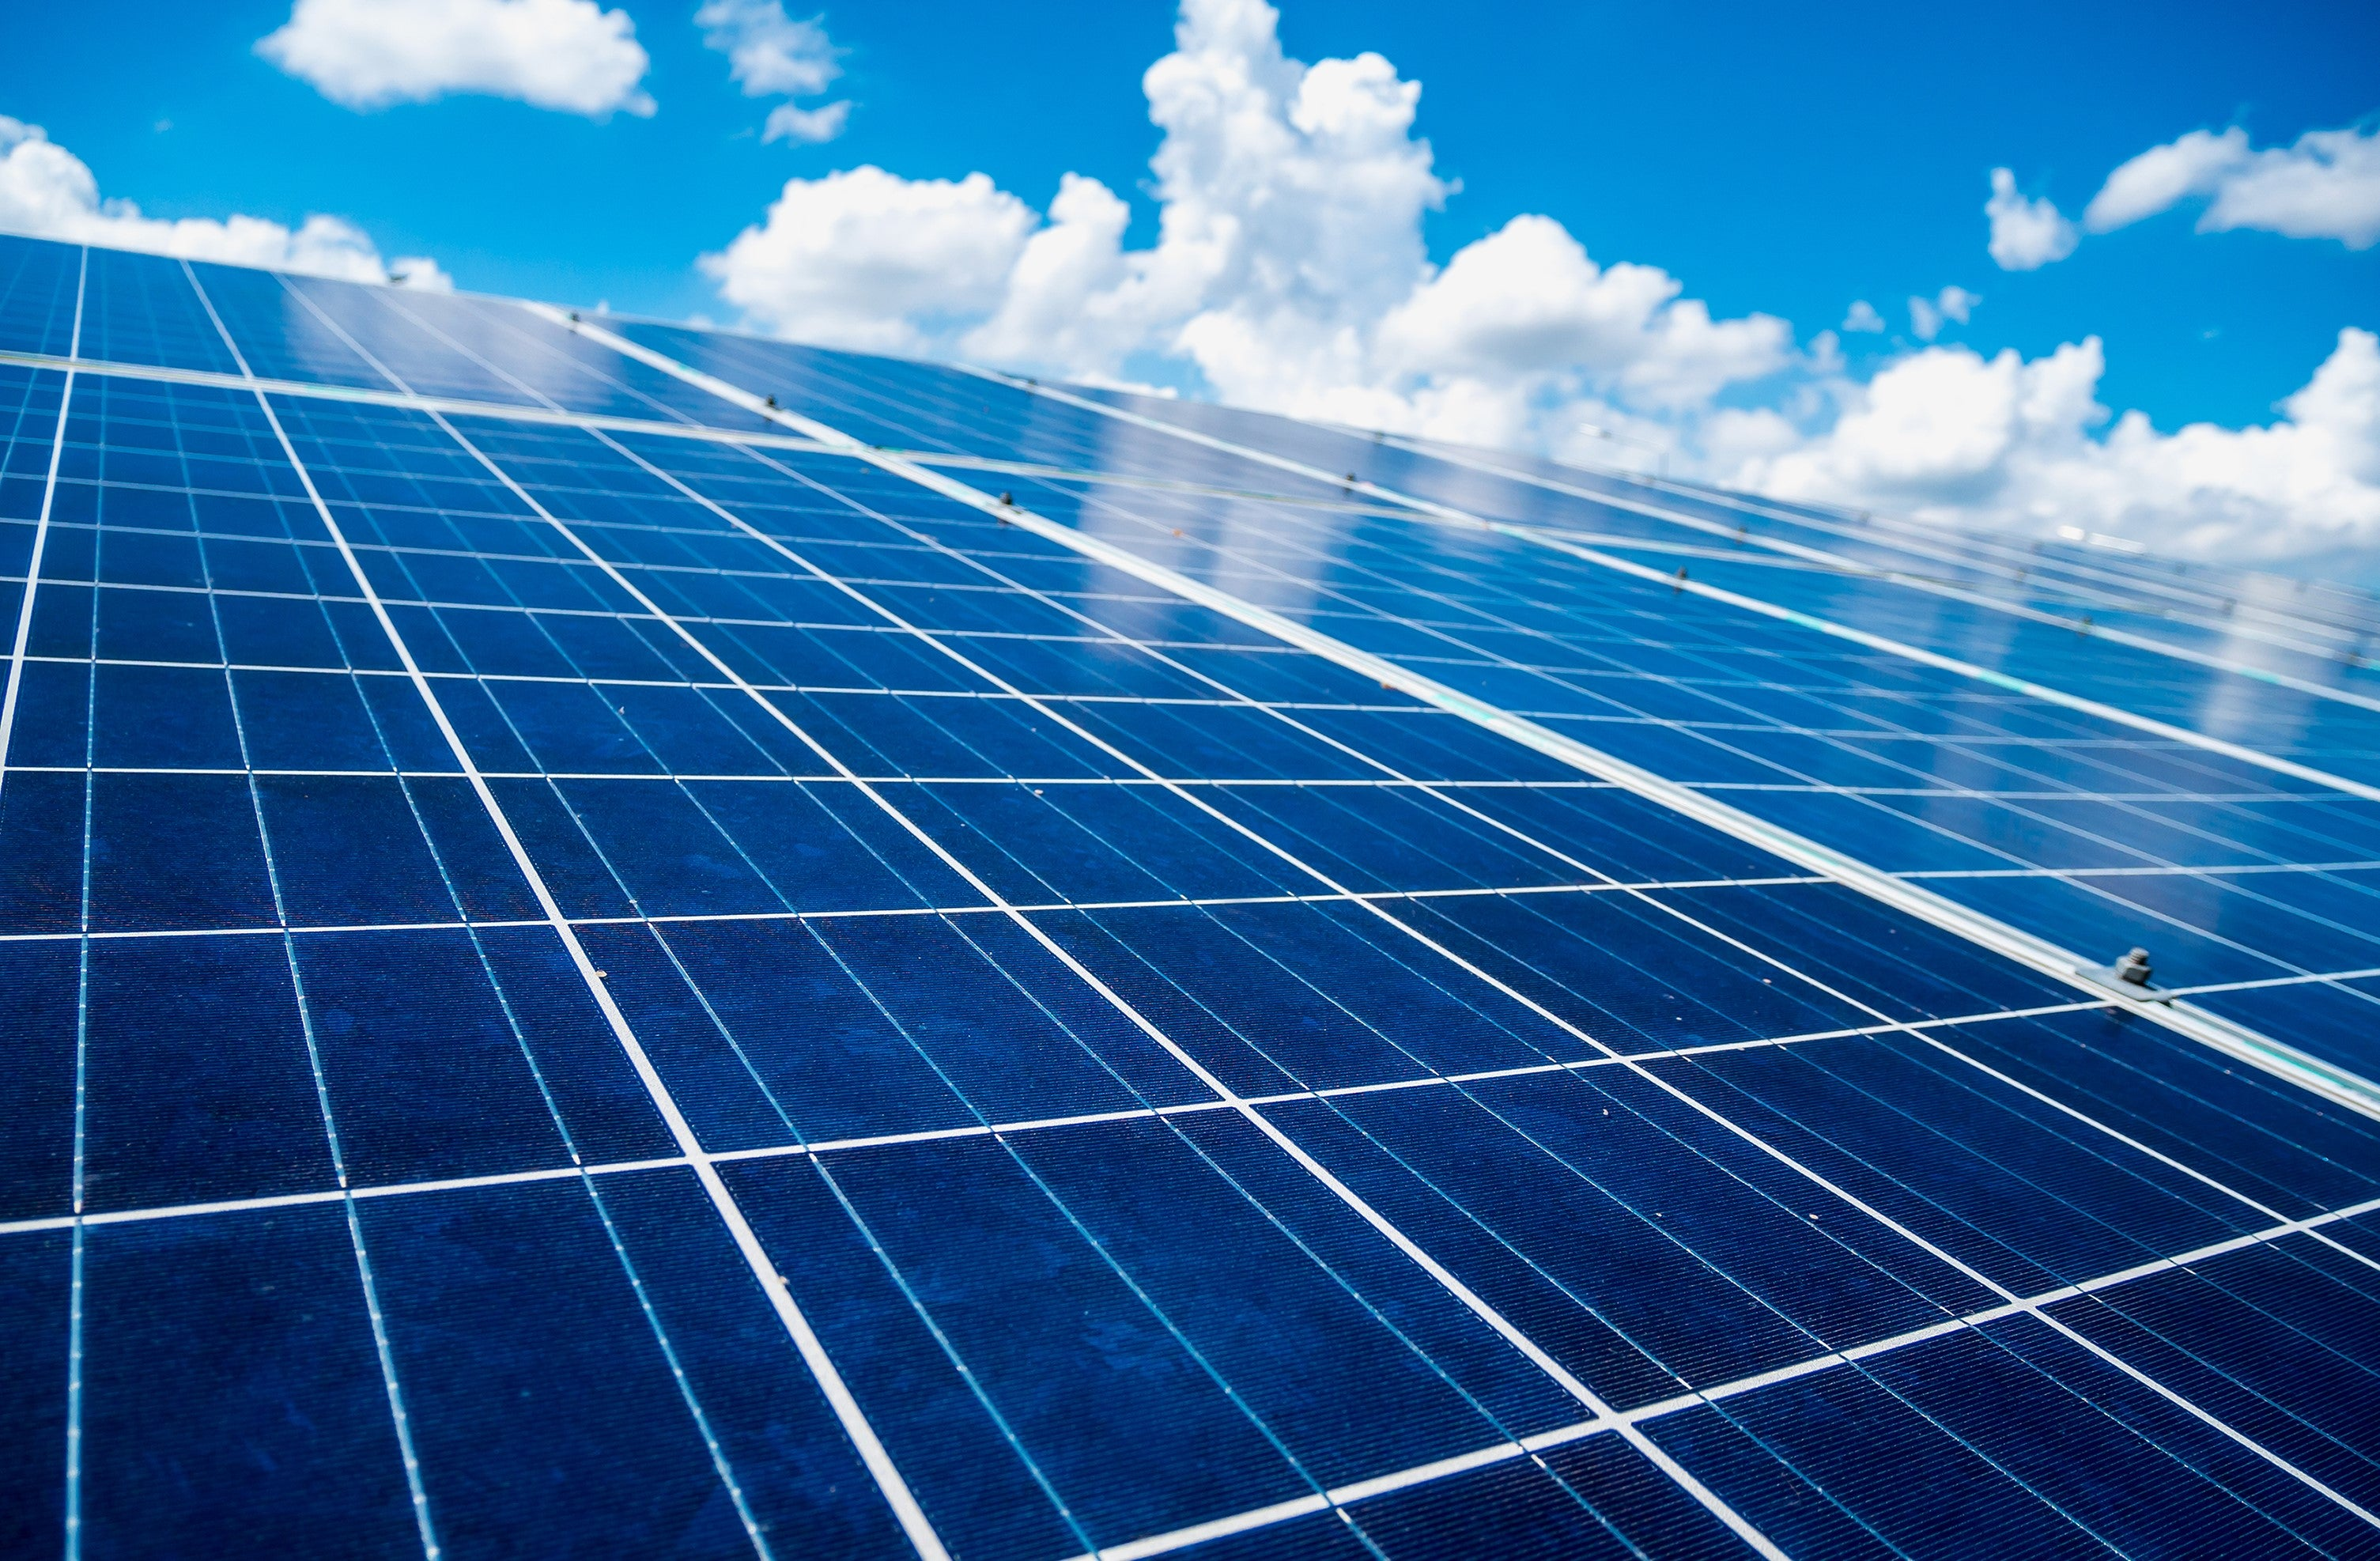
\includegraphics[width=5.5cm]{sections/0_intro/imgs/plant.jpg}
	\end{wrapfigure}

	However, these data often contain gaps and deficiencies.

	Accurate imputation of these gaps is essential to ensure the reliability of analyses and predictions based on this data.
	%        The growing need for the adoption of tools capable of generating clean energy from renewable and sustainable sources has led to extensive generation and collection of energy production data, especially from photovoltaic panels installed worldwide.
	%        
	%        However, these data often have gaps and deficiencies due to various factors such as temporary failures, adverse weather conditions, or malfunctions of sensors and data collection instruments.
	%    
	%    Accurate imputation of these gaps is crucial to ensure the reliability of analyses and predictions based on this data. 
\end{frame}